\section{Template-based Programming model}\label{sec:model}

\begin{figure}[tp]
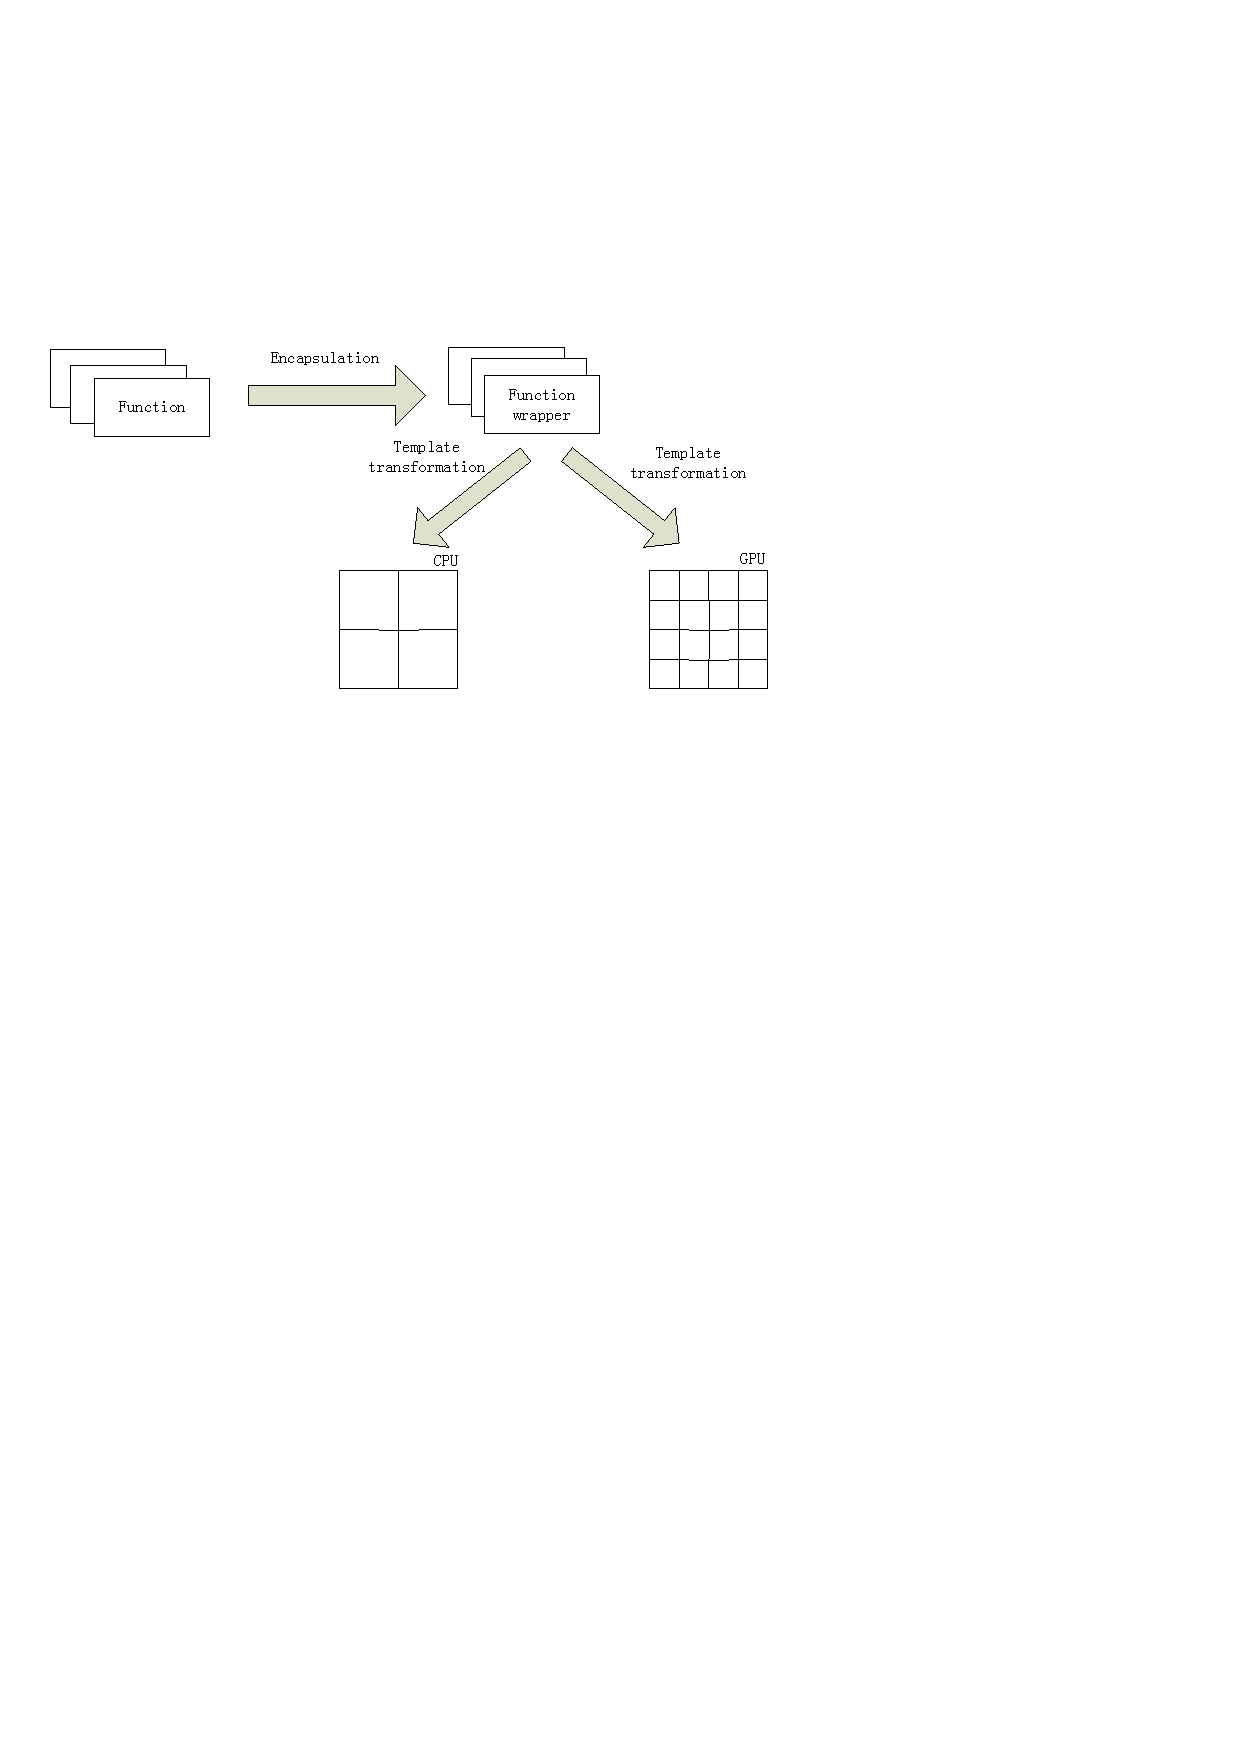
\includegraphics[width=3.3in, height=4.0in]{../overview}
\caption{Overview of template-based programming model: Programers
write side-effect free functions in C/C++, then encapsulate them into
function wrappers. Template library regards a function wrapper as
a task. Tasks are transformed into a
group of subtasks based on appropriate parallel patterns, finally map tasks on physical multicores.}\label{fig:overview}
\end{figure}

\hspace{-1ex}\begin{figure}[tp]
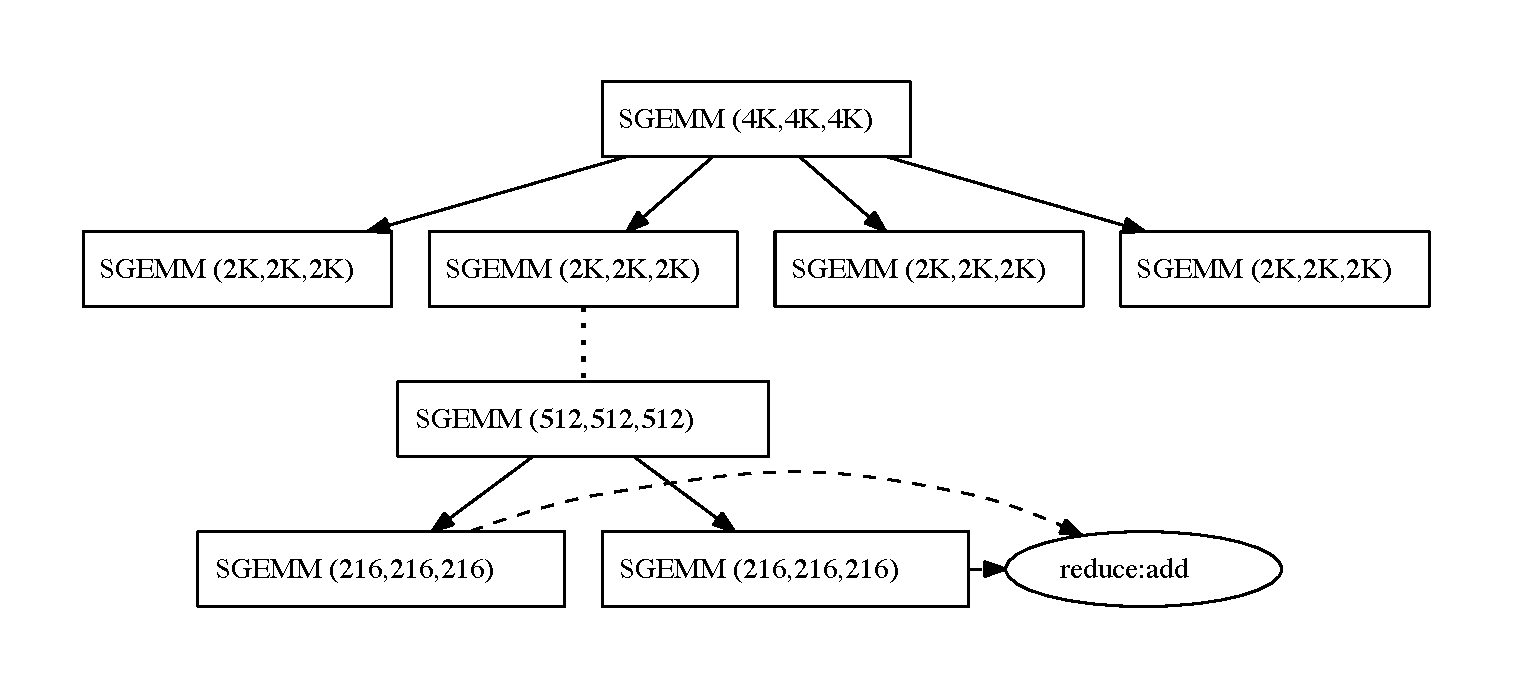
\includegraphics[width=3.5in]{../mmexample}
\caption{Matrix-multiplication(sgemm) division:Divide 
matrix-multiplication task into smaller subtasks. The division process
is implemented by List. 1. Triple in figure represents
task parameters (M, P, N), which means A[M][P] * B[P][N]. The figure
is the result of parameterizing K = 2. } \label{fig:mmexample}
\end{figure}

%programming model
We use template metaprogramming to implement a parallel programming model.
Essentially, our approach utilizes C++ template mechanism to
perform source-to-source transformations for multicores. Side-effect
free functions are abstracted as \emph{tasks}. A task is
wrapped in the form of template class, named \emph{function
  wrapper}.  A \emph{TF class} is a template class, which
is capable of transforming a task into a group of subtasks based on
a parallel pattern. Tasks
apply TF classes according to their appropriate
parallel patterns. This process is called ast \emph{adaption}. 
Finally, we use \emph{building block classes} to define executions of tasks
on specific architectures. Both TF classes and building
blocks are organized as a library --
\textbf{libvina}. Fig.~\ref{fig:overview} depicts the diagram of template
library-based programming model. Conventional functions are
encapsuated into function wrappers. After transformation at compile time, they are
executed on different multicore architectures at run time.

\renewcommand\linenumberfont{\normalfont\small}
\setlength\linenumbersep{-0.06in}

%\lstset{language=C++}
%\lstset{breaklines}
%\lstset{extendedchars=false}
%\lstset{numbers=left, numberstyle=\tiny}


%\begin{lstlisting}
%\makebox[3.4in]{\hrulefill}

%\linenumbers
%\begin{verbatim}
%\end{verbatim}
%\nolinenumbers
%\begin{figure}[hbt]
  \inputsrc{sgemm.cc}
  %\caption{Example of pseudo-code of the patching library.}
  %\label{patch_lib}
%\end{figure}

%\end{lstlisting}\label{lst:mm}
\makebox[3.4in]{\hrulefill}

List 1 Example code of sgemm: SGEMM class adapts TF\_hierarchy
to implement \emph{Divide-and-Conquer} algorithm of matrix
multiplication. Function \textit{innner} at
line 20 divides task into subtasks, while function \textit{leaf} at
line 45 performs
computation. Call operator function at line 14 is the user interface for the task.
Line 24$\sim$37 is lambda expression to perform map/reduce, corresponding to
SGEMM(512, 512, 512) node in Fig.~\ref{fig:mmexample}\\

\inputsrc{langpipe.cc}
\makebox[3.4in]{\hrulefill}

List 2  Example code of langpipe: A translation is a standalone
function wrapper. TF class synthesizes a pipeline. \\

%Building blocks \textit{par} and \textit{reduce} to express execution.
Programmers using our template-based programming model are free to
choose ways to parallelize tasks. An example applying 
Sequoia's programming model is shown in Fig.~\ref{fig:mmexample}. 
\textit{sgemm} is a task to perform matrix-mulitplication. 
We can apply a TF class dedicated to hierarchical division.  List 1
illustrates the adaption. As a reuslt, we
implement the straightforward \emph{Divide-and-Conquer} algorithm for
sgemm, which divides a matrix into K*K
submatrices, computes them recursively, and reduces the results for
each division.
The control flow of source transformation is programmed
using template metaprogramming inside of the TF class. 
To demonstrate the more than one way of parallelization can be
achieved in our programming model, List 2 gives pipeline processing example, which is similar to Streamit. It implements language translation pipeline by
synthesizing a pipeline of four standalone functions. TF\_pipeline is a TF class
representing time-multiplex parallelism. As shown in examples,
the parallel patterns and execution models are dramatically
different, however, our approach can describing them well in uniform
language constructs.

%meaning
Our programming model facilitates the separation of roles in software
development. Algorithm-centric programmers are only concerned of algorithm
in conventional C/C++ form, as at line 45 of List 1 and line 8 of
List 2. On the other side,  system programmers knowing underlying
architectures are in charge of developing and
applying template classes to specialize tasks for the specific
targets. This separation not only simplifies the difficulties of writing and
tuning parallel programs, but also facilitates to develop effecient and
portable programs for various multicores.


%section end.